\chapter{Evaluation}
\label{CHAP_SIXTH}
\centerline{\rule{149mm}{.02in}}
\vspace{2cm}

\section{Implementation / Results Summary}
\subsection{Qualitative Analysis}

The main result of the qualitative analysis was of great compliment to OpenStack. Overall, it appears to be a well designed system, which exhibits all of the desired characteristics of a Cloud and of a Virtual Infrastructure Manager. By analysing the architecture and design of the system using standard metrics such as cohesion, it was possible to form a coherent conclusion about OpenStack which would provide useful perspective on it's workings. The below figure shows which of the desired characteristics of a VIM and of a cloud are covered by which components of OpenStack, giving an overview of \textit{how} OpenStack provides the services and capabilities required of each: 
\begin{figure}[ht]
\centering
\fbox{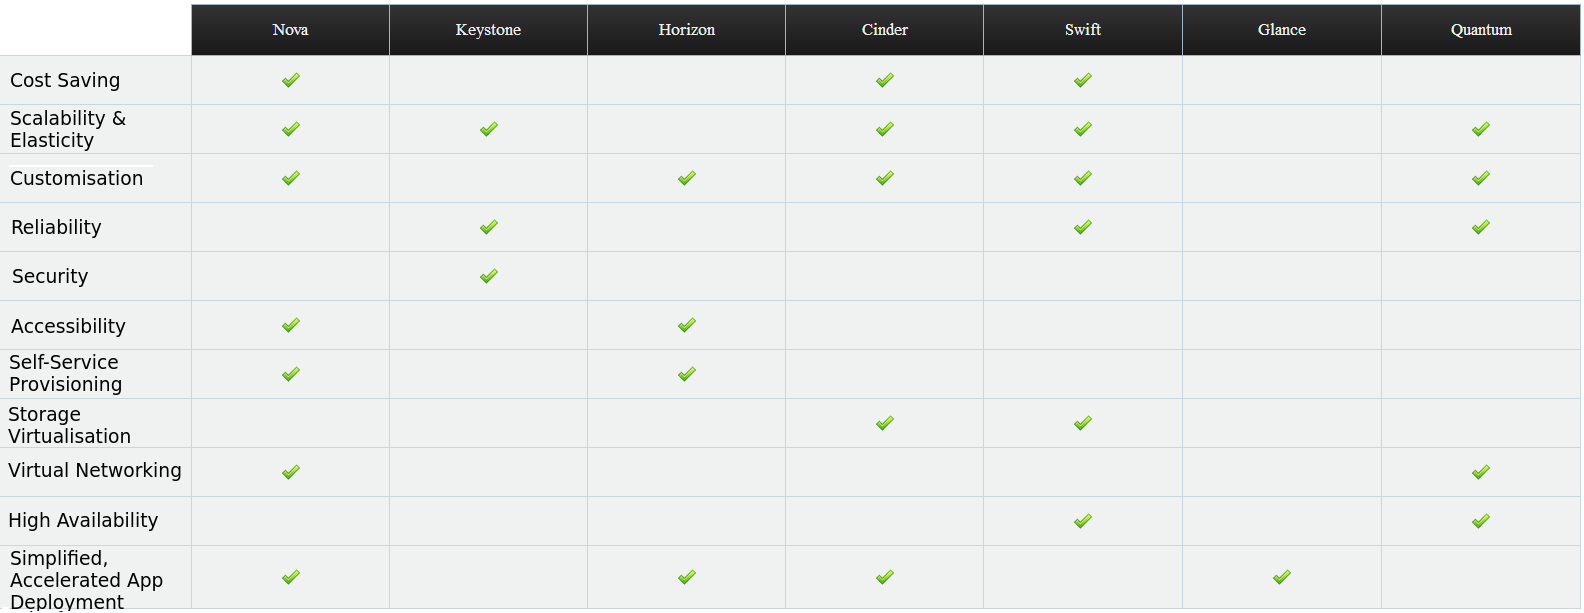
\includegraphics[scale=0.24]{cloud-characteristic-comparison}}
\caption{Table showing which Desired Cloud \& VIM Characteristics are exhibited by which OpenStack components, based on this project's Qualitative report}
\end{figure}
Overall, in terms of cohesion and coupling, it was found that OpenStack has a very well defined modular design, which allows for components to be highly cohesive and act as services to the other components, together forming an effective system. This was shown in most components by the narrow aims and capabilities of each module. For example, the Glance Image service would exclusively handle bootable VM Images, and try not to go beyond that. 
However, in places this granularity did cause some problems, as there seemed to be some conflict between the decoupled mentality, and the ability to make certain modules self-sufficient. The most salient example of this was the Nova module, which, despite being a specialised Virtual Machine Instance management module, had its own concepts and definitions of VM images and networks, meaning that it had very low cohesion. The idea here was clearly to allow basic setups based around the Keystone and Nova modules, meaning there was no heavy dependency on other modules to provide services, but in the end this caused inconsistencies in the application when those modules handling each were involved. A great example of this was the REST APIs for the Nova \& Glance components. each had its own definition of what an Image was, and for a client, it became increasingly confusing to actually use both of these modules together. In the end, the result was that the Glance service was not relied on, as nova provided its own version of this functionality. 
These drawbacks are far outweighed by the flexibility and customisation provided by the loosely-couple architecture, and the use of standards-compliant RESTful APIs make interaction between components extremely simple. It appears, from this analysis at least, that the designers of OpenStack made the right decision to go in a new direction and go with a fine granularity based approach, as this provides a number of advantages for clients deploying their own instances of OpenStack. 
Another feather in the cap of OpenStack uncovered by this analysis was the sheer level of customisation and functionality available through its various components. Even given the high level of expectation in terms of functionality on a system which provides cloud infrastructure, OpenStack delivers; advanced features such as Software Defined Networking, Virtual Storage, and high availability object storage are provided, meaning that, on paper, it is a perfectly viable cloud solution. 

 

\subsection{Qualitative \& Quantitative Experiments}
The results of the 'Exploring OpenStack through Experimentation' section were very mixed. In some cases, experimentation was very informative, and brought useful information to light. A 'conclusion' section can be found at the end of each given experiment, explaining the results and how they are interpreted. In this section, I will reflect on the overall results of running experiments; what was achieved, whether the experiments were useful, and what they mean for somebody using OpenStack. \\
The first 'type' of experiment ran, of which there were three (K1, N1, N2), were the 'Validator Experiments', the aim of these being to not only validate OpenStack functionality, but also to develop a reusable client for this functionality, and even to give a brief review of it, in terms of metrics such as conceptual complexity, or code complexity. These experiments were very successful. For each piece of functionality, the experiments provide background information about how they work, and then guide the reader through the development process for both the functionality itself and the validator experiment, with code then being provided as a guide for further development, as well as a re-usable testing component. All of this is valuable to somebody wishing to learn how to interact with OpenStack, and even somebody wishing to validate their own deployment. In each case, the developed functionality worked well, and this functionality was then cleared for use in the later quantitative experiments.   It is my view that this level of useful product justifies the 'validation' approach.\\
The 'Quantitative Performance Experiments', of which there were two (N3, N4), provided a totally different angle for OpenStack analysis. These were much more practical, and were devised in the hopes of testing OpenStack for characteristics such as Scalability, Elasticity, and Efficient Resource Allocation. These experiments proved to be much more challenging to execute, mainly due to unexpected resource limitations, discussed later in this chapter (Unexpected Issues/Limitations). These limitations meant that many of the results, particularly for the Server Launch Experiments, were partial, and so it was difficult to effectively draw conclusions from the results in a reliable manner. Due to this, the conclusions made were kept limited, and the Experiments provided as re-usable code for those users with larger deployments to try for themselves. Another issue was with the interpretation of results. In some cases, certain behaviour could only be observed, and not necessarily explained, due to a lack of time and lack of knowledge of the inner workings of OpenStack. Despite these issues, the experiments, along with experiment K2, a practical security test, uncovered some very useful information, which can be found at the end of each experiment write up under the 'Conclusion' heading, and so I believe that they were still worth executing. It would have been a good idea to design experiments with the resource limits in mind, but unfortunately I was not aware of them at design time, and such a drastic change in approach was not possible at such short notice. \\
Some interesting findings from these experiments are listed below:
\begin{itemize}
\item The OpenStack Keystone Identity service can be deployed 'unsecured' over plain HTTP, which is VERY dangerous in multi-tenant deployments. An experiment successfully intercepted packets containing private authentication information.
\item OpenStack Nova Compute scales well with respect to number of VMs launched simultaneously and also with respect to launching a VM with current load, although less so.
\item OpenStack Nova Compute does a good job of scaling in terms of 'Flavor Size' or VM resource allocation size, as results show many operations are not slowed down at the same rate as the increase in size of the VM. For example, m1. medium is approximately 4x the size of m1 small, and yet operations are not 4 times slower. 
\item Suspending a Server is a lower performance, less scalable solution for stopping the running of a server when compared to pausing and locking a server; it is however necessary if RAM is limited on the cluster.  
\end{itemize}

\subsection{Delivered OpenStack Client}
This project has delivered a working OpenStack client. The first main aim of this client was of course, to interact with OpenStack's REST APIs to perform various actions. In this sense, it was of course successful, in that it performed multiple actions on 3 of OpenStack's components; Nova, Keystone and Glance, with a 100\% success rate. This client functionality was then exposed through a number of Java interfaces in order to be used by any client, or experiment, that requires it.\\
The consequence of this is the satisfaction of the second, and arguably most important aim of the client; to validate OpenStack functionality. Experiments were successfully created using the aforementioned interfaces, and tested the effects of each successful interaction. In this way, we validated that OpenStack behaves as expected, and also does so on the Leeds Test Bed deployment, something which is a useful basis for further experimentation. \\
One of the greatest achievements of this code however is that it is designed to be easily re-usable. The use of Spring's JavaBean XML definitions for OpenStack configuration and Experiments allows any OpenStack setup and written experiments to be executed. A base class for new experiments which allows them to hook into this system is also provided; all of this is explained in Appendix E. From this, it is clear that what has been delivered is a means to use OpenStack, create experiments for further testing, execute experiments old or new, and learn about how to develop for the REST APIs. I would therefore deem this an overall success. \\
However, there were some issues with this deliverable. Firstly, as with the  experiments, it was not possible to cover much of OpenStack, due to the various limitations discussed later in this chapter. Secondly, due to time constraints, full and expanded documentation was not possible, and so much of the code must be read and understood without much guidance.  Perhaps the biggest problem with the development was due to the nature of REST APIs; asynchronous requests created certain delays which are not handled by the REST API. This did seem to be a failing of the design of the API, not including some kind of job context which would be used to query the status of a job. The closest thing to this was the status code of each request, but a 200 OK code would not guarantee there was not an issue, and utilities like those in the \textit{NovaUtils} class were necessary to make up for this. For example, if a Server is launched, a 200 OK response code does not imply the server is not in 'Error' state. There would also be problems that if a Server was deleted, it would still show up if a request to list active servers was sent, as the delete operation was not completed. The utility methods \textit{waitForServerState} and \textit{waitForServerDelete} were created to tackle each of these respectively.

\subsection{Conclusion}

From the discussion above, I would suggest that the results and deliverables from this project have provided useful and varied information about OpenStack. Through the Qualitative report, there is good coverage of OpenStack despite limitations, and I believe that it would really help a user learn about it at a high level. To complement this, and make up for its natural 'high level information only' limitation, experiments both qualitative and quantitative provide more specific details about OpenStack's APIs, functionality and performance in a real deployment. Although not all of OpenStack was covered, arguably its two most vital parts, Keystone and Nova, were. The experiments have been delivered in code form, along with a code deliverable which allows for anyone to set up and execute them, plus their own experiments, with minimal configuration. It is plain to see that I have not only experimented, but paved the way for further experimentation and development in this area. \\
Overall, it appears to have been a good to have three separate deliverables. Each of these could of course be improved upon, and that is certainly something for the future which will be discussed later in this chapter, but overall, I am happy that enough information and guidance has been delivered concerning OpenStack. 

\section{Comparison with other Evaluations}

As part of the Evaluation of this Evaluation of OpenStack, it is important to compare it against the previous evaluations which were highlighted in the background research for this project. In this way, we can ascertain whether this project has added any value to the domain, and have some point of comparison to gauge the relative success of the project. 

\subsection{ETF Evaluation}
In some ways, the ETF evaluation\cite{etfevaluation} \& this one bear similarity. For example, both initially aim to provide a basic overview of the OpenStack technology; the ETF evaluation starts with a list of relevant components of OpenStack, to give the high level view, as does this. They are also similar in that they both aim to provide insight and guidance as to the use of OpenStack, something at least in part covered in this evaluation. Where these two differ, however, is that there is a particular focus on User Experience and Deployment in the ETF evaluation, something not covered in this evaluation. On the other hand, this evaluation covers aspects of OpenStack that the ETF did not, such as the performance of the Nova compute component \& comparing interfaces to OpenStack. In this sense, I believe this evaluation does cover new ground, and provide new information and knowledge.  
Similarly, it seems the approach of my evaluation was much more in depth than that of the ETF; certain aspects, such as 'architecture', which were analysed in depth using formal metrics in this report, were covered in a one sentence answer by the ETF. In general, this evaluation is longer and more in depth, giving me confidence that this report will be useful. 
The final difference spotted was the lack of development involved in the ETF evaluation. There is no evidence of programmatic experimentation being documented by their evaluation. Furthermore, a toolset ready made from Eucalyptus, a competitor project, was used instead of the approach of this project, which was to develop a client specifically for OpenStack. 
One thing this has shown me is that I may have been able to get more done in terms of experimentation and analysis if I too had used a ready made tool to interact with OpenStack. This is perhaps a failing on my part, not knowing the true benefit of the standards-compliant REST APIs OpenStack employs. \\
In terms of results consistency, there were some joint findings. The main example of this is the issue of security, where both evaluations found, albeit in different ways, that there was some issue with the identity service. 

\subsection{CERN Evaluation}
Before a comparison is made between the CERN evaluation\cite{cernevaluation} mentioned, it is important to mention that the actual findings of this report were not made available, and so what will be compared is the \textit{approach} of the CERN evaluation, not its results. 
In aims and objectives, it appears that the CERN evaluation was heavily focussed on the validation of OpenStack's functionality; something that was also covered in this evaluation. Another common goal of each project was the practical use of OpenStack as a form of analysis and this validation. In this sense, CERN's evaluation seems to go into further detail than this evaluation, which is more focussed on basic usage. I believe this is mainly down to the resources allocated to each project; it was difficult to perform advanced manipulation of the resources given, as described in the  'Unexplained issues/limitations' section of this evaluation. Despite this, I still believe that the 'guide' style of this project's validation is useful, and it does cover some functionality that is not highlighted by CERN, such as server metadata and keystone authentication. 
To further compare the two, it is worth noting that CERN had some qualitative evaluation planned, but the focus was more on administrative functionality like provisioning hardware and managing the VM lifecycle, not analysis of the design and architecture of OpenStack, as in this evaluation, so this project does cover new ground in this sense. However, CERN did not include any form of pure quantitative evaluation, for example, performance testing, nor did they intend to produce a code deliverable similar to the REST Client delivered here. In this way, my evaluation is providing new value to the domain. One aspect of the CERN evaluation I could really learn from is the great level of planning. Every step of the project was clearly mapped out early on, something which was not the same for this evaluation, although the resources and aims of this project were always less clear from the off. Due to this, it is my view that the CERN evaluation was a better structured, more organised approach to OpenStack's evaluation.

\subsection{Conclusion}
Overall, it seems that this evaluation of OpenStack has provided some real value to the OpenStack knowledge base, and hopefully to members of the ASCETiC team, and other readers. The coverage of OpenStack was high qualitatively, but some detailed analysis was still possible quantitatively, providing a good balance of the level of information. I feel that in places, this project has covered new ground, and gone into more detail on other areas, such as programmatic experimentation. 

Provided below is a table comparing what is provided by each evaluation:

\begin{figure}[H]
\centering
\fbox{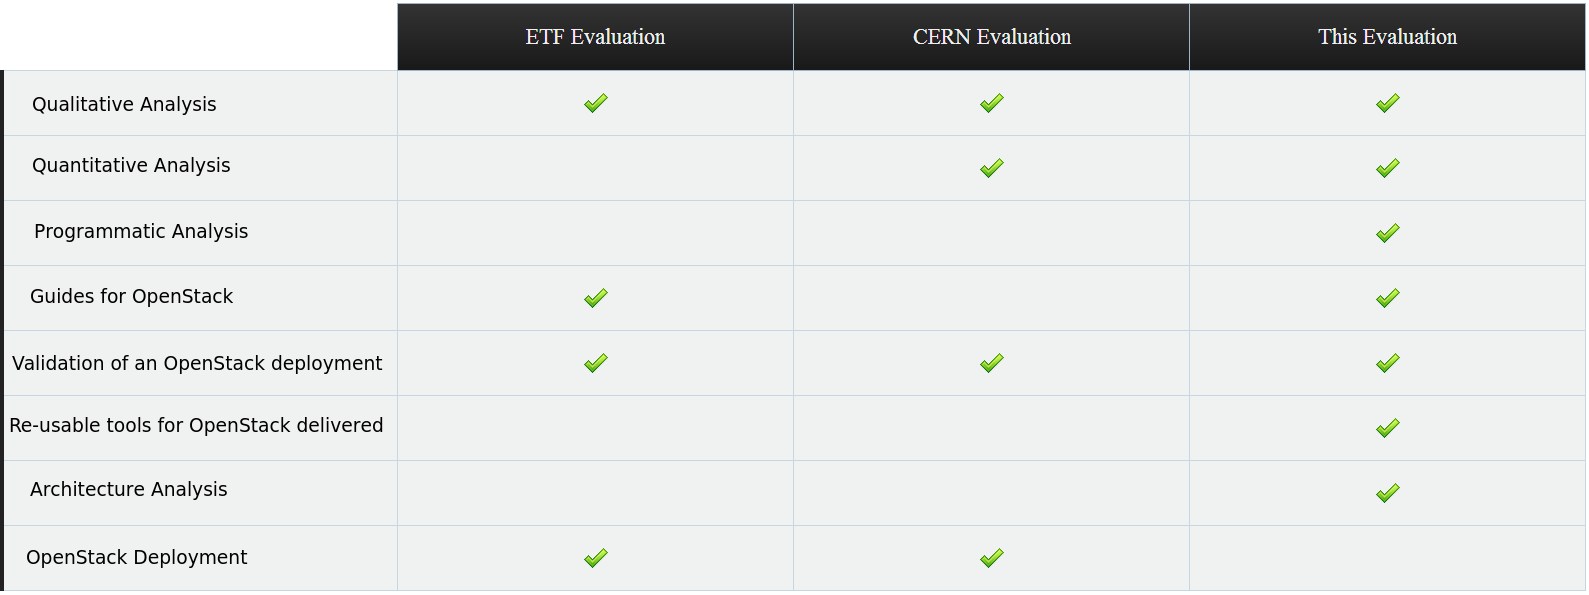
\includegraphics[scale=0.24]{evaluation-comparison-table}}
\caption{Table showing which aspects of Evaluation are covered in each evaluation, comparing this project with 2 previous evaluations.}
\end{figure}

I am happy with the performance of my evaluation in this table, as it shows that it covered a great number of aspects which one or the other previous evaluation did not, and in some cases, new ground entirely. In a space which is relatively new, it may indeed be one of the first of these reports of its kind. One issue I have had with the results is perhaps the 'jack of all trades' approach; by this I mean that qualitative analysis, quantitative experimentation and software development were all combined into the project, where maybe it would have been possible to focus on one. This approach came from a couple of real aims; firstly, was to cover new ground, especially in the practical, quantitative space. Given the limitations discussed later in this chapter, and the aim to provide guidance to OpenStack, it made a lot of sense to infuse example code and analysis of OpenStack with this too, to give an example of how to deal with OpenStack in a number of ways, practically and theoretically. I really feel like the project was successful in this respect.  

\section{Project Management \& Outcome}
\subsection{Aims \& Objectives}
In light of the outcomes of this project, I am a firm believer that the aims \& objectives of this project were well set, and were reasonably difficult, but still achievable. Having objectives as varied as those for this project was always going to be a risk; it was hard to know how long each would take, given that there was no clear information about OpenStack or its use at the time. The idea then was to attempt to link these objectives together, so that much of the work would in some way contribute to multiple aims. For example, the objective of producing implementations for programmatic tests and the other to produce re-usable software were always intended to be intertwined, and the resulting REST Client reflects this. The aims \& objectives of the project were not necessarily clear at the start of the project, however, and were slightly modified as a response to the feedback from my mid-project report. The feedback stated that the objectives were perhaps unclear or vague, and so I felt it important to consider 'what is an evaluation'? This process can be read at the end of the 'Background Research' section, where the plan for evaluation of OpenStack is explained. \\
In conclusion, I am happy with the way the objectives looked after the initial re-think. Initially, they were perhaps too vague, such as 'Produce an evaluation report of OpenStack' with no explanation. Changing this to 'Produce a Qualitative Architecture \& Functionality Analysis' meant that it was clear what the aim of the deliverable was, and these changes as a whole helped to really form the identity of the project. 

\subsection{Project Methodology}
As mentioned in Chapter 1 of this report, the approach to this project was defined in 2 ways. Firstly, it would take an agile approach, meaning development would be incremental and formed as it was developed, using rapid prototyping techniques. Secondly, it would be split into four phases; research, implementation, conclusion and evaluation.  \\
The agile approach in itself has proved itself as the correct choice for this type of project. As the objectives and amount of work to be done were unclear, the approach of developing ever-improving prototypes meant that the code and report were not sensitive to changes in the project definition at any one time, and were always ready to be delivered if time ran out. Working in sprints personally helped my focus, and whole experiments could be completed in short bursts of effort, helping to organise the project work effectively. The iterative approach is not well reflected in the resuts write-up, and this is mainly because the iterations were very small and part of the developemnt process, not something I deemed worthy of write-up.  Splitting the work into 'phases' went hand in hand with the approach just mentioned. I was able to give myself free reign to work on what was needed, and be incredibly flexible, as long as project milestones were hit. All research was completed before implementation began, and all implementation finished before conclusions were drawn, etc. Within each of these phases, what work was to be done was kept loosely defined, with a list of work to do always available. This was particularly helpful due to the learning nature of the project. If I was stuck on developing the report, I could switch to developing the code deliverable, and this often taught me more about what I needed to know about OpenStack for the report. \\
Neither of these approaches were without problem. The approaches were indeed flexible, but in some cases this meant being unorganised, and often it was easy to lose track of what work was completed and needed completion, especially after a break from work. Despite this, the outcome of the project justifies the approach in my opinion, and I am happy that the work was consistently productive throghout, partly down to these approaches. 

\subsection{Project \& Time Management}
The way the project was managed has no doubt helped to make it successful. The approach in general was to work on an ad-hoc, flexible basis so as to simultaneously work on multiple deliverables, and this put a lot of emphasis on how my time and the workload were managed. 
A useful tool I used was a simple Note Taking application on my laptop. When work was to be done, this would be written up as a task list, and struck off when it was completed. By looking through this and the work, it was easy for me to guage where the most work needed to be done, and from this I could decide where to place my effort. 
Tools such as version control on this LateX project and every code deliverable meant that work could be completed anywhere, on multiple machines at home or university, something which had a huge effect on my time management, as I could work whenever I needed to without waiting, and more effectively and flexibly perform sprints.
My approach was tested part-way through the project when the requirements changed, and so much of the time and energy that would be spent on work by my GANTT chart were spent almost 're-defining' the project. It is testament to the methodology and the management of the project that this did not affect the final outcome, and putting in more hours, and perhaps scaling back on the more advanced objectives, solved this issue. 
In terms of time management, I do think there are some things I could have improved upon. For example, the testing of prototypes was not something I spent enough time on, and this often meant spending more time fixing problems in the code than was necessary. Problems like this were down to my own failings, wanting to do the more exciting work most of the time, and neglecting other work. Unlike many projects, this report was written as the project went on, and iteratively developed like the other deliverables, as opposed to just being written up at the end, meaning I could ensure a slightly higher level of quality than there would have been if it were rushed at the end. 
Due to changes in the project, and a few personal problems, the look of my GANTT chart did change, mainly taking longer and with planning in the middle. The updated chart can be found in Appendix F: 

\subsection{Unexpected Issues/Limitations}
\begin{itemize}
\item Cinder \& Swift could not be installed due to a lack of LVM technology on servers.
\item Neutron could not be installed due to incompatibility with the Leeds network
\item Hardware resources were limited to 2 machines, 8gb RAM, 8 cores. 
\item Didn't have full admin access to OpenStack until late in the project
\item Server Migration could not be performed as both OpenStack servers had different architectures. 
\item Time taken to deploy OpenStack ate into early project time.
\item No comparable setup was available to evaluate another product in comparison quantitatively. 
\item Documentation for OpenStack was often found lacking, especially for feature explanations.
\end{itemize}

\section{Future work} 
\subsection{Further Research}


The possibility of future work in this area is almost limitless due to the size of OpenStack, but with more time I would have focussed on first including the final two missing components from the qualitative analysis, Ceilometer and Heat\cite{openstacksoftware} to improve coverage. Next, I would have performed more investigation of the design, including new metrics such as static code analysis, bug count and code coverage. Finally, a full architecture and capability analysis comparison with another project such as OpenNebula is something I would have aimed for, in order to assess OpenStack vs the competition.

\subsection{Further Experiments}
The first work that follows from this is to of course run the designed experiments on a larger OpenStack deployment, to get some more useful results at larger scale. Following this, I would have aimed to have the other OpenStack components, such as Cinder, installed, and validator experiments created for each, to validate their functionality. Once validated, the possibility for experimentation is endless, but some key experiments I aimed for were performance analysis of server migration and scalability of storage creation using Cinder. I also aimed to compare the launch of a VM when using a snapshot vs using a bootable VM image. Luckily, the way the experiment framework is written allows for these types of experiments to be developed relatively easily, and this was in mind when designing the framework. 

\subsection{Improving the REST Client library}
Before talking about the next parts of this tool to be developed, it is important to mention a couple of improvements that could be made. Firstly, updating the current clients to new APIs would be useful, as some were just being released as the project went on. Secondly, the authentication system could be improved to include validation of a token and knowledge of when tokens time out; much information is provided with a response from Keystone, such as timeout date, but this project only uses the token itself at this point. Finally, the documentation of the code could be massively improved, and is not at its best due to the rapid development approach taken. Further work would of course include developing client functionality for other components in order to create experiments, but also improvements to the Exception handling of the project, in order to more effectively handle errors with OpenStack. Further utilities would also need to be created in order to handle any other issues with new REST APIs. 

\section{Conclusion}

This chapter has aimed at evaluating the work performed in the previous chapter by first summing up the results and findings, and then assessing those results, through comparison with previous similar projects, and by other means.  Furthermore, it has critically evaluated the project approach and management as a whole, considering which aspects were successful and unsuccessful, and finally, what work would have been performed had there been more time. The idea of this chapter was to give some insight into the nature of the project, what it was like to work on, and what issues were discovered and potentially overcome. \\

The next, and final chapter of this report considers whether the initial aims and objectives of the project have been met or exceeded, as this is one of the most salient indicators of success.    